\section{Originalità introdotte}
In questa sezione vengono riportate le originalità che abbiamo ritenuto significative e che abbiamo voluto introdurre nella relazione, ripartite per algoritmo.

\subsection{Held-Karp}
Mobilitati da curiosità abbiamo provato a variare il tempo di calcolo a disposizione dell'algoritmo di Held e Karp, per vedere se le soluzioni che impiegavano più di due minuti ritornavano una soluzione migliore, oppure se, con meno tempo a disposizione, la soluzione ritornata risultava peggiore. Le tabelle sottostanti riportano quello che è stato ottenuto.

\subsubsection{Held-Karp con 1 minuto}
\begin{center}
	\begin{longtable}{|c|c|c|c|}	
	\hline
		\multirow{2}{*}{\textbf{Istanza}} & \multicolumn{3}{c|}{\textbf{Held-Karp}} \\ \cline{2-4}
		 &\textbf{Soluzione}& \textbf{Tempo (s)} & \textbf{Errore (\%)} \\ \hline
		\endfirsthead
		\multicolumn{4}{|c|}%
		{\tablename\ \thetable\ \ --\  \textit{continuazione della pagina precedente}} \\
		\hline
		\multirow{2}{*}{\textbf{Istanza}} & \multicolumn{3}{c|}{\textbf{Held-Karp}} \\ \cline{2-4}
		 &\textbf{Soluzione}& \textbf{Tempo (s)} & \textbf{Errore (\%)} \\ \hline
		\endhead
		\hline \multicolumn{4}{|r|}{\textit{Continua nella pagina seguente}} \\
		\endfoot
		\endlastfoot
berlin52 & 17441 & 60,706 & 131,25 \\ \hline
burma14 & 3323 & 0,1014 & 0,00 \\ \hline
ch150 & 47935 & 59,999 & 634,29 \\ \hline
d493 & 111947 & 60,598 & 219,83 \\ \hline
dsj1000 & 551274242 & 60,001 & 2854,35 \\ \hline
eil51 & 986 & 60,000 & 131,45 \\ \hline
gr202 & 55127 & 60,000 & 37,26 \\ \hline
gr229 & 176212 & 59,999 & 30,91 \\ \hline
kroA100 & 165018 & 60,000 & 675,38 \\ \hline
kroD100 & 146158 & 59,999 & 586,38 \\ \hline
pcb442 & 202517 & 59,999 & 298,82 \\ \hline
ulysses16 & 6859 & 0,3550 & 0,00 \\ \hline
ulysses22 & 7013 & 53,181 & 0,00 \\ \hline
		\caption{Risultati dell'algoritmo Held-Karp concedendo 1 minuto}
	\end{longtable}
\end{center}\vspace{-40pt}
\subsubsection{Held-Karp con 5 minuti}
\begin{center}
	\begin{longtable}{|c|c|c|c|}	
	\hline
		\multirow{2}{*}{\textbf{Istanza}} & \multicolumn{3}{c|}{\textbf{Held-Karp}} \\ \cline{2-4}
		 &\textbf{Soluzione}& \textbf{Tempo (s)} & \textbf{Errore (\%)} \\ \hline
		\endfirsthead
		\multicolumn{4}{|c|}%
		{\tablename\ \thetable\ \ --\  \textit{continuazione della pagina precedente}} \\
		\hline
		\multirow{2}{*}{\textbf{Istanza}} & \multicolumn{3}{c|}{\textbf{Held-Karp}} \\ \cline{2-4}
		 &\textbf{Soluzione}& \textbf{Tempo (s)} & \textbf{Errore (\%)} \\ \hline
		\endhead
		\hline \multicolumn{4}{|r|}{\textit{Continua nella pagina seguente}} \\
		\endfoot
		\endlastfoot
berlin52 & 17441 & 303,951 & 131,25 \\ \hline
burma14 & 3323 & 0,15270 & 0,00 \\ \hline
ch150 & 47935 & 316,682 & 634,29 \\ \hline
d493 & 111947 & 308,136 & 219,83 \\ \hline
dsj1000 & 551274242 & 306,492 & 2854,35 \\ \hline
eil51 & 984 & 300,463 & 130,98 \\ \hline
gr202 & 55127 & 305,269 & 37,26 \\ \hline
gr229 & 176212 & 312,290 & 30,91 \\ \hline
kroA100 & 162606 & 308,605 & 664,05 \\ \hline
kroD100 & 144125 & 314,625 & 576,83 \\ \hline
pcb442 & 202044 & 300,972 & 297,89 \\ \hline
ulysses16 & 6859 & 0,40430 & 0,00 \\ \hline
ulysses22 & 7013 & 57,7751 & 0,00 \\ \hline
		\caption{Risultati dell'algoritmo Held-Karp concedendo 5 minuti}
	\end{longtable}
\end{center}\vspace{-40pt}
\subsubsection{Held-Karp con 10 minuti}
\begin{center}
	\begin{longtable}{|c|c|c|c|}	
	\hline
		\multirow{2}{*}{\textbf{Istanza}} & \multicolumn{3}{c|}{\textbf{Held-Karp}} \\ \cline{2-4}
		 &\textbf{Soluzione}& \textbf{Tempo (s)} & \textbf{Errore (\%)} \\ \hline
		\endfirsthead
		\multicolumn{4}{|c|}%
		{\tablename\ \thetable\ \ --\  \textit{continuazione della pagina precedente}} \\
		\hline
		\multirow{2}{*}{\textbf{Istanza}} & \multicolumn{3}{c|}{\textbf{Held-Karp}} \\ \cline{2-4}
		 &\textbf{Soluzione}& \textbf{Tempo (s)} & \textbf{Errore (\%)} \\ \hline
		\endhead
		\hline \multicolumn{4}{|r|}{\textit{Continua nella pagina seguente}} \\
		\endfoot
		\endlastfoot
berlin52 & 17441 & 603,349 & 131,25 \\ \hline   
burma14 & 3323 & 0,15163 & 0,00 \\ \hline
ch150 & 47885 & 606,479 & 633,53 \\ \hline
d493 & 111947 & 603,658 & 219,83 \\ \hline
dsj1000 & 550719964 & 611,369 & 2851,38 \\ \hline
eil51 & 963 & 601,293 & 126,05 \\ \hline
gr202 & 55125 & 605,391 & 37,26 \\ \hline
gr229 & 175982 & 603,008 & 30,74 \\ \hline
kroA100 & 161443 & 699,899 & 658,58 \\ \hline
kroD100 & 143960 & 605,555 & 576,05 \\ \hline
pcb442 & 202044 & 603,171 & 297,89 \\ \hline
ulysses16 & 6859 & 0,40640 & 0,00 \\ \hline
ulysses22 & 7013 & 58,3268 & 0,00 \\ \hline
		\caption{Risultati dell'algoritmo Held-Karp concedendo 10 minuti}
	\end{longtable}
\end{center}\vspace{-40pt}

\subsubsection{Conclusioni}
La variazione del tempo concesso per il calcolo dell'algoritmo \texttt{HeldKarp} non ha avuto alcun miglioramento né peggioramento per sei istanze di TSP su tredici. Per tre di loro, precisamente \texttt{burma14.tsp, ulysses16.tsp e ulysses22.tsp}, questo accade perché la soluzione ottima viene già trovata entro un intervallo di tempo relativamente basso, quindi non considerato perché ritenuto poco interessante: la più \quotes{impegnativa} delle tre, \texttt{ulysses22.tsp}, è in grado di ritornare la soluzione ottima in poco meno di un minuto. Le altre due in meno di un secondo.\eqcapo
Per quanto riguarda le rimanenti sette istanze di TSP, vale a dire \texttt{ch150.tsp, dsj1000.tsp, eil51.tsp, gr202.tsp, gr229.tsp, kroA100.tsp, kroD100.tsp} invece si è registrato un aumento della qualità della soluzione ritornata, all'aumentare del tempo di computazione concesso. I grafici sottostanti riportano i dati inseriti nelle tabelle di cui sopra, mostrando più chiaramente la differenza degli errori relativi calcolati come $(SoluzioneTrovata - SoluzioneOttima)/SoluzioneOttima$,  ripartito in base alle diverse tempistiche assegnate.
\paragraph*{ch150.tsp}
\image{0.7}{ch150}{Variazione dell'errore relativo in ch150}
\paragraph*{dsj1000.tsp}
\image{0.7}{dsj1000}{Variazione dell'errore relativo in dsj1000}
\paragraph*{eil51.tsp}
\image{0.7}{eil51}{Variazione dell'errore relativo in eil51}
\paragraph*{gr202.tsp}
\image{0.7}{gr202}{Variazione dell'errore relativo in gr202}
\textbf{Nota:} in questo grafico, essendo troppo piccola la variazione, i due valori riportati sull'asse delle ordinate vanno sommati con il numero scritto in notazione scientifica in alto a sinistra.
\paragraph*{gr229.tsp}
\image{0.7}{gr229}{Variazione dell'errore relativo in gr229}
\paragraph*{kroA100.tsp}
\image{0.7}{kroA100}{Variazione dell'errore relativo in kroA100}
\paragraph*{kroD100.tsp}
\image{0.65}{kroD100}{Variazione dell'errore relativo in kroD100}
\mbox{}\eqcapo

Come ci si poteva aspettare, concedendo più tempo di computazione all'algoritmo \texttt{HeldKarp}, abbiamo registrato una probabilità non banale che l'algoritmo migliori le sue \emph{performance}: 
\begin{itemize}
	\item Non considerando le tre istanze di TSP in cui l'algoritmo riesce a trovare la soluzione ottima sotto al minuto, si rimane quindi con dieci istanze: \texttt{berlin52.tsp, ch150.tsp, d493.tsp, dsj1000.tsp, eil51.tsp, gr202.tsp, gr229.tsp, kroA100.tsp, kroD100.tsp} e \texttt{pcb442.tsp}.
	\item Sette di loro hanno un miglioramento della soluzione ritornata $\Rightarrow$ \textbf{70\%} delle possibilità che \texttt{HeldKarp} restituisca una soluzione più vicina alla soluzione ottima all'aumentare del tempo concesso.
\end{itemize}
Seppure ci sia chiaro che non sia corretto derivare giudizi generali di qualsiasi tipo avendo a disposizione così poche istanze di TSP, riteniamo di aver ottenuto una percentuale davvero alta, di cui si debba tenere conto, risultato sperimentale che conferma ciò che ci aspettavamo.\acapo

Crediamo che, alla luce di quanto detto finora, sia il caso di chiederci: vale la pena concedere fino a dieci minuti per trovare una soluzione migliore?
\begin{itemize}
	\item La risposta che ci siamo dati è, non sorprendentemente, \textbf{dipende}: se il grafo ricavato dall'istanza di TSP possiede un numero di nodi $n$:
	\begin{itemize}
		\item $0< n \leq 22 $ allora assegnare più tempo a \texttt{HeldKarp} \textbf{è indifferente}, in quanto l'algoritmo ritorna una soluzione ottima in meno di un minuto (quindi si ferma in ogni caso);
		\item $23 \leq n < 52$ allora assegnare più tempo a \texttt{HeldKarp}\textbf{ probabilmente non conviene}, perché impiegando invece l'euristica \texttt{CheapestInsertion} si ottengono risultati statisticamente migliori (vedi tabella \ref{tab}). Ad ogni modo, occorre precisare che per valori di $n$ immediatamente successivi a 22, invece, \textbf{probabilmente conviene} lasciare più tempo all'algoritmo, perché potrebbe ritornare una soluzione ottima entro 10 minuti.
		\item $ n\geq 52$ allora assegnare più tempo a \texttt{HeldKarp} \textbf{sicuramente non conviene}, perché abbiamo sperimentato che, per ogni istanza di TSP, risultati migliori si possono ottenere impiegando l'euristica \texttt{CheapestInsertion}.
	\end{itemize}
\end{itemize}

\subsection{CheapestInsertion e TriangularTSP}
Entrambi gli algoritmi sono una 2-approssimazione per TSP, ma riportano risultati differenti: \texttt{CheapestInsertion} richiede più tempo per essere eseguito rispetto a \texttt{TriangularTSP}, ma ottiene un errore relativo minore.\acapo 
Per capire dunque quale dei due algoritmi sia più efficiente ed efficace, è possibile osservare gli istogrammi in Figura~\ref{confronto} che mostrano prima la differenza del tempo di esecuzione dei due algoritmi su scala logaritmica per i vari grafi, poi il tempo di esecuzione su una scala normale ed infine il rispettivo errore relativo. Confrontando il primo e terzo istogramma è possibile vedere come per un aggiunta di tempo di computazione relativamente basso si ottiene un notevole miglioramento per l'errore relativo, infatti \texttt{TriangularTSP} raggiunge in media un errore relativo più alto ($\sim$32\%) rispetto a \texttt{CheapestInsertion} ($\sim$16\%). Se si osserva il secondo istogramma si può vedere come con grafi di taglia maggiore il tempo di esecuzione per \texttt{CheapestInsertion} aumenti esponenzialmente rispetto a \texttt{TriangularTSP}, basti osservare il tempo di esecuzione per i grafi \textit{d449} e \textit{dsj1000}. \acapo

Dunque per grafi di grande taglia è consigliabile utilizzare \texttt{TriangularTSP}, altrimenti \texttt{CheapestInsertion}.

\begin{figure}
	\centering
	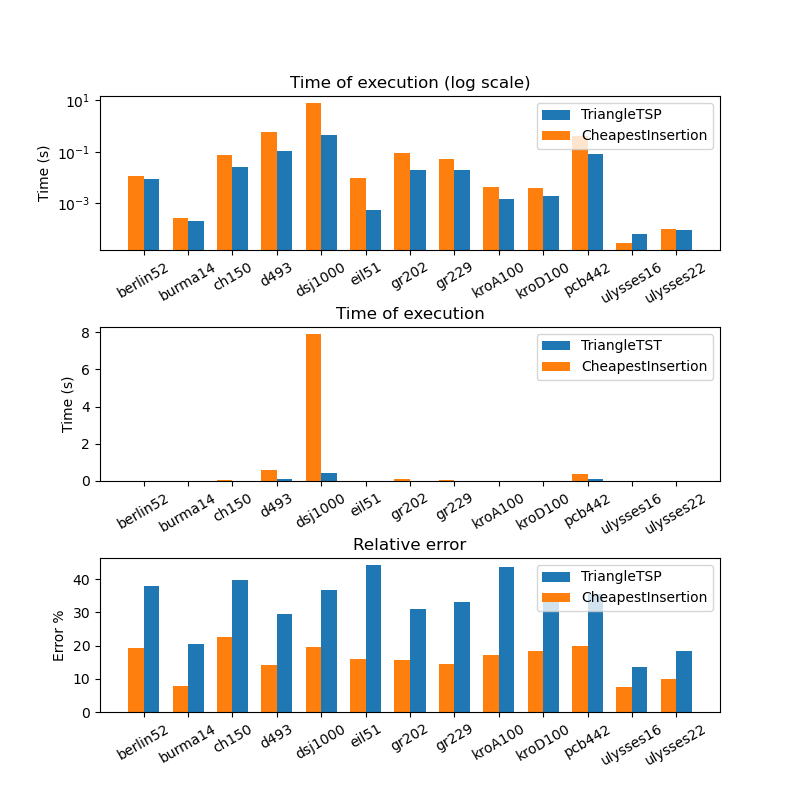
\includegraphics[width=\textwidth]{confronto}
	\caption{Confronto tra \texttt{CheapestInsertion} e \texttt{TriangularTSP}}
	\label{confronto}
\end{figure}
